
% android_app.tex

\chapter{Android-App: ApoCo}

Dieses Kapitel beschriebt die Android-App.
Sie dient dem an Adipositas erkrankten Patienten als \"Ubersicht und Eigenkontrolle f\"ur sein Essverhalten und K\"orperlichen-Zustand.
Der App-Projektname lautet \emph{ApoCo}. Er ist von der Bezeichnung \emph{Adipositas-Controlling} abgeleitet.
Die App wird in diesem Kapitel durch Designentscheidungen in der Architektur, GUI und Implementierung beschrieben.



\section{Modellierung}

Die Software ist stark modularisiert und dom\"anenorientiert aufgebaut.
Wichtige Aspekte, die zu dieser Entscheidung gef\"uhrt haben, sind unter anderem,
dass die Software sp\"ater einfach und schnell erweitbar, \"anderbar und partiell wiederverwendbar sein soll.
Die Modularisierung erfolgt nach Funktionen und Teilaufgaben innerhalb einer Funktion.
ApoCo wird mittels verschiedener Architekturen realisiert.
Zun\"achst ist die grobe Struktur der Android-Anwendung als \emph{Model-View-Controller (MVC)} modelliert.
Die einzelnen Schichten Model, View und Controller der Android-Anwendung sind wie in der Abbildung 4.1 aufgeteilt.\\

\begin{figure}[h]
  \centering
  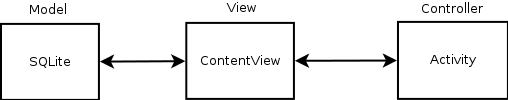
\includegraphics[scale=0.7]{diagramme/kapitel4/MVC.png}
  \caption{MVC-Architektur der ApoCo-Anwendung}
 
\end{figure}

\begin{itemize}
 \item Model: Die Model-Schicht ist die interne Datenbank der ApoCo-Anwendung.
 Als Datenbank nutzt Android SQLite.
 Dabei ist die Datenbank als eine Datei umgesetzt.
 Diese ist auf dem Dateisystem in Ordnern der ApoCo-Anwendung hinterlegt.
 Die Anfragen und Statements werden hier genauso verwendet wie das zum Beispiel der Fall bei MySQL oder Oracle Datenbanken ist.
 
 \item View: Die View-Schicht wird durch die \emph{Views} einer Android-Activity repr\"asentiert.
 Eine solche View wird in den meisten F\"allen in einer XML-Datei beschrieben.
 Diese Datei enth\"alt die Struktur einer View, welche dem Benutzer anschlie\ss{}end auf dem Bildschirm pr\"asentiert wird.
  
 \item Controller: Die Controller-Schicht wird durch die Anwendungslogik in den Activities umgesetzt.
 Hier wird die Interaktion des Patienten mit ApoCo abgefangen und die Ausgaben f\"ur den Bildschirm gesteuert.
\end{itemize}


Wird das gesamte Projekt betrachtet, handelt es sich dabei um eine Client-Server-Architektur.
In der Abbildung 4.2 wird die Aufteilung der einzelnen Software-Komponenten der Client-Server-Architektur dargestellt.\\

\begin{figure}[h]
  \centering
  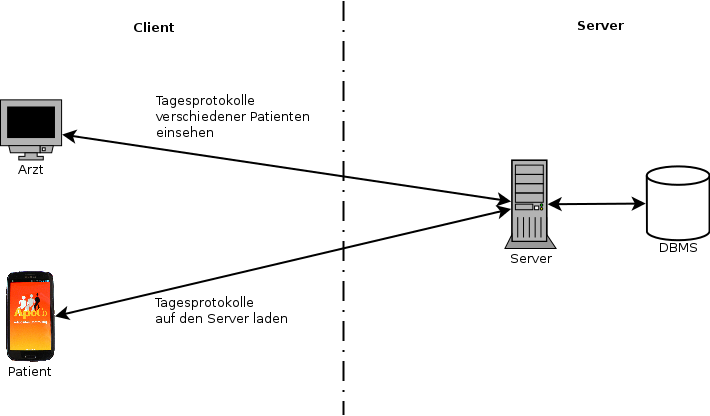
\includegraphics[scale=0.5]{diagramme/kapitel4/client_server.png}
  \caption{Client-Server-Architektur des gesamten Projekts}
  
\end{figure}

ApoCo ist der Teil der gesamten Software, welcher sich um das Aufzeichnen von Tagesprotokollen k\"ummert.
Um die Daten auswerten zu k\"onnen, benutzt der Arzt eine Webanwendung.
Dabei werden die Tagesprotokolle von der Datenbank geladen und im Webbrowser des Arztes angezeigt.\\
 

% \section{Modelierung}
% 
% Die Software ist stark modularisiert und Dom\"anen orientiert aufgebaut.
% Der Grund daf\"ur ist, die Software soll sp\"ater einfach und schnell erweitbar und \"anderbar sein.
% Die Modularisierung erfolgt nach Funktionen und Teilaufgaben innerhalb einer Funktion.
% ApoCo wird mittels verschiedener Architekturen realisiert.
% Zu n\"achst ist die grobe Struktur der Android-Anwendung als \emph{Model-View-Controller (MVC)} modeliert.
% Die einzelnen Schichten Model, View und Controller der Android-App sind wie in der Abbildung 4.1 aufgeteilt.
% 
% \begin{figure}[h]
%   \centering
%   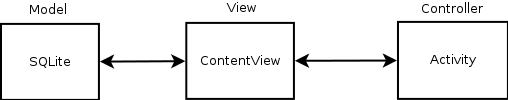
\includegraphics[scale=0.7]{diagramme/kapitel4/MVC.png}
%   \caption{MVC-Architektur der ApoCo-Anwendung}
%  
% \end{figure}
% 
% \begin{itemize}
%  \item Model: Die Model-Schicht ist die interne Datenbank der ApoCo-App.
%  Als Datenbank nutzt Android SQLite.
%  Dabei ist die Datenbank in Form einer Datei umgesetzt.
%  Diese ist auf dem Dateisystem in Ordnern der ApoCo-App hinterlegt.
%  Die Zugriffe auf diese Datenbank entsprechen zum gro\ss{}en Teil MySQL.
%  
%  \item View: Die View-Schicht wird durch \emph{ContentViews} einer Android-Acctivity representiert.
%  Ein solcher Content wird in den meisten F\"allen in einer XML-Datei beschrieben.
%  Diese Datei h\"allt die Struktur einer View, welche sich dem Benutzer anschlie\ss{}end auf dem Bildschirm presentiert.
%   
%  \item Controller: Die Controller-Schicht wird durch die Anwendungslogik in den Activities umgesetzt.
%  Hier wird die Interaktion des Patienten mit ApoCo abgefangen und die Ausgaben f\"ur den Bildschirm gesteuert.
% \end{itemize}
% 
% 
% Wird das gesammte Projekt betrachtet handelt es sich dabei um eine Client-Server-Architektur.
% In der Abbildung 4.2 wird die Aufteilung der einzelnen Software-Komponennten in der Client-Server-Architektur dargestellt.
% 
% \begin{figure}[h]
%   \centering
%   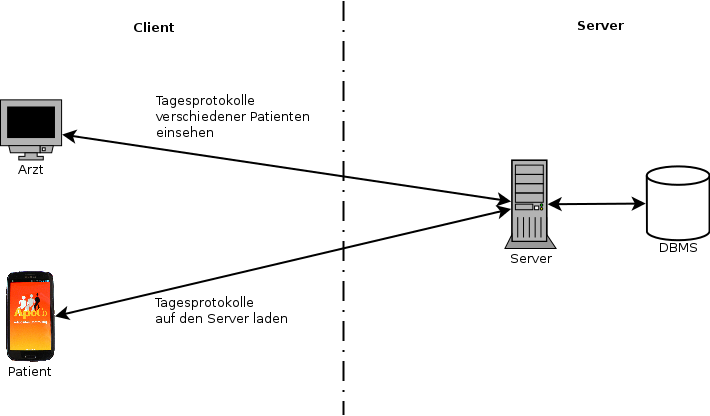
\includegraphics[scale=0.5]{diagramme/kapitel4/client_server.png}
%   \caption{Client-Server-Architektur des gesammten Projektes}
%   
% \end{figure}
% 
% ApoCo ist der Client der Software welcher sich um das aufzeichnen von Tagesprotokollen k\"ummert.
% Um die Daten auswerten zu k\"onnen benutzt der Arzt eine Webanwendung.
% Das ist der Client f\"ur den Arzt, der sich mit dem Server verbindet und einen Zugriff auf die Tagesprotokolle des Patienten erlaubt.


\section{Apoco Projektstruktur}

Die Abbildung 4.3 veranschaulicht die Paketstruktur der ApoCo-Anwendung.
Sie spiegelt die Modularisierung der ApoCo-Anwendung wieder.
Im Ordner \emph{src} befindet sich der gesamte Quellcode der Anwendung. 
Dieser liegt aufgeteilt in den jeweiligen Modul-Paketen im Hauptpaket der Anwendung \emph{com.janas.apoco}.\\

\subsection*{Paket activity}

Das Paket \emph{activity} beinhaltet alle f\"ur die ApoCo-Anwendung notwendigen Activities.
In diesem Paket befinden sich folgende Klassen:

\begin{itemize}
 \item ActivityBloodpressure:\\
 Hier steht die gesamte Anwendungslogik f\"ur das Protokollieren von Blutdruck.
 Die Activity veranschaulicht in einer scrollbaren Liste alle vorhandenen Messungen.
 Dar\"uber hinaus werden die Daten beim Verlassen der Activity \"uber das Internet mit einem Webserver synchronisiert. 
 
 \item ActivityBodyweight:\\
 Diese Activity behandelt das Protokollieren von K\"orpergewicht des Patienten und beinhaltet die daf\"ur notwendige Anwendungslogik.
 Auch hier werden in einer Listenansicht alle get\"atigten Messungen angezeigt.
 Beim Beenden der Activity werden die Protokolle mit einem Webserver synchronisiert.
 
 \item ActivityDeviceList:\\
 Diese Activity ist notwendig f\"ur das Koppeln \"uber Bluetooth von Sensoren mit dem Smartphone.
 Es ist eine von zwei M\"oglichkeiten des Koppelungsvorgangs in der ApoCo-Anwendung.
 Hier verh\"alt sich das Smartphone wie ein Client.
 Die Activity hat zwei Listen.
 In der einen Liste werden bereits bekannte Ger\"ate aufgelistet.
 Nach einem erfolgreichen Suchvorgang werden die gefundenen Ger\"ate in der zweiten Liste angezeigt.
 Man w\"ahlt aus einen der Listen das gew\"unschte Ger\"at zum Koppeln aus und sie verbinden sich untereinander.
 
 \item ActivityDevices:\\
 Diese Activity bietet die M\"oglichkeit den Koppelungsvorgang zu starten.
 Man w\"ahlt die Art des Messger\"ats aus, zum Beispiel K\"orperwaage, Blutdruckmesser oder Lebensmittelwaage.
 Anschlie\ss{}end w\"ahlt man die Koppelungsart aus.
 Zur Auswahl stehen die M\"oglichkeiten \emph{als Server} und \emph{als Client} zur Verf\"ugung.
 Die Methode \emph{pairing als Client} wird mittels der Klasse ActivityDeviceList ausgef\"uhrt.
 Die Methode \emph{pairing als Server} erledigt die ActivityDevices selbst.
 Daf\"ur startet sie einen Thread mit einem BluetoothServerSocket.
 Dieser h\"ort auf Anfragen von externen Ger\"aten zum Koppeln.

 \item ActivityFoodKcal:\\
 Hier wird der Benutzer drauf aufmerksam gemacht, wieviele Kilokalorien er am aktuellen Tag bereits zu sich genommen hat.
 Zus\"atzlich wird die erlaubte Restmenge berechnet und dem Benutzer angezeigt.
 Wird die erlaubte Tagesdosis \"uberschritten, erscheint eine Warnung auf dem Display.
 In einer Liste werden vorhergehende Mahlzeiten aufgelistet.
 Beim Klicken auf eine Mahlzeit wird die Activity \emph{ActivityMealenergyDetails} als \emph{Dialog} eingeblendet und listet die einzelnen
 Positionen der Mahlzeit mit Informationen \"uber Energie und Gewicht auf.
 Von hier aus gelangt der Benutzer weiter zur Protokollierung einer neuen Mahlzeit und zur Ger\"ate-Koppelung.
 
 \item ActivityMealenergy:\\
 Beim Start ist die Activity immer leer.
 Der Benutzer st\"o\ss{}t von hier aus den Protokollierungsvorgang an.
 \"Uber den Barcode-Button startet der Benutzer eine Activity f\"ur das Scannen von EAN-Codes.
 Anschlie\ss{}end wird eine interne und externe Datenbank nach der gescannten EAN-Nummer durchgesucht.
 Wird ein Eintrag gefunden, so wird der Benutzer zur Activity \emph{ActivityMealContent} weitergeleitet, sonst wird eine Fehlmeldung ausgegeben, dass das Lebensmittel
 nicht identifiziert werden konnte.

 \item ActivityMealenergyContent:\\
 In diese Activity gelangt man nur, wenn das Lebensmittel in der Datenbank identifiziert wurde. 
 Hier werden Detailinformationen \"uber das Lebensmittel angezeigt 
 und \"uber den Button \emph{Waage verbinden?} kann eine Verbindung zur Lebensmittelwaage ge\"offnet werden. 
 
 Nach erfolgreicher W\"agung errechnet die Activity die Energiemenge des gewogenen Lebensmittels, 
 die Gesamtenergie aller Mahlzeiten und
 die noch zur Verf\"ugung stehende Energiemenge f\"ur den aktuellen Tag.

 \item ActivityMealenergyDetails:\\
 Diese Activity erscheint lediglich im Stil eines \emph{Dialog}.
 Das bedeutet, dass die alte Activity im Hintergrund sichtbar bleibt  
 und der modale Dialog tritt wie ein Pop-up in den Vordergrund. 
 Sie besteht nur aus einer scrollbaren Liste und zeigt Details einer Mahlzeit auf.
%  \item ActivityFoodKcalNewEntry:\\

 \item ActivityLogin:\\
 Diese Activity dient dem Anmelden in der ApoCo-Anwendung.
 Alternativ kann ein neuer Benutzer zur Activity \emph{ActivityRegister} wechseln, um sich zu registrieren. 
 
 \item ActivityRegister:\\
 Die Activity tritt als modaler Dialog auf und dient der Erfassung eines neuen Benutzers.
 Hier tr\"agt der Benutzer seine Daten wie Vor- und Nachname, Email und Passwort ein.
 Die Activity f\"uhrt eine Plausibilit\"atskontrolle durch.
 Anschlie\ss{}end sendet sie die Daten an einen Webserver, welcher \"uberpr\"uft, 
 ob der Benutzername bereits vergeben ist. 
 Sollte der Name zur Verf\"ugung stehen, wird der Benutzer in die Datenbank aufgenommen, 
 andernfalls wird er abgelehnt. 
 Die Activity reagiert auf die Serverantwort und akzeptiert entsprechend die Benutzerdaten 
 oder fordert ihn erneut auf seine Eingabe zu \"uberarbeiten.
 
 \item ActivityServerOptions:\\
 Diese Activity erscheint als modaler Dialog und nimmt lediglich die Adresse und Port des Webservers entgegen.
 
 \item ActivitySplashscreen:\\
 Das Splashscreen wird beim Start von ApoCo f\"ur wenige Sekunden angezeigt.
 Diese Activity pr\"asentiert das Logo und den Schriftzug \emph{(Adipositas Controlling}.
 Die Activity beendet sich nach einem Timerablauf automatisch und startet die Start-Activity von ApoCo.

 \item ActivityStart:\\
 Das ist die Hauptactivity in der ApoCo-Anwendung.
 Hier w\"ahlt man die Art der Protokollierung aus.
 Das kann zum Beispiel eine K\"orpergewichtsmessung, Blutdruckmessung oder das Protokollieren der eigenen Nahrungsaufnahme sein.
 Dar\"uber hinaus hat der Benutzer von hier aus den Zugriff auf die Funktion zum Koppeln von Messsensoren.

 %  \item ActivitySummary:\\
\end{itemize}



\begin{figure}[h]
  \centering
  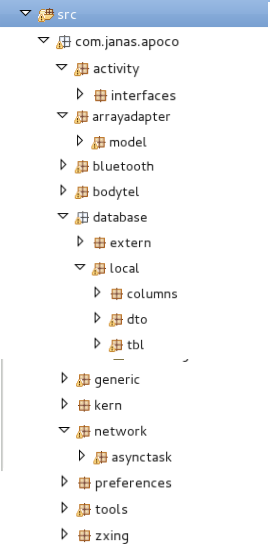
\includegraphics[scale=0.7]{screenshots/kapitel4/projekt_struktur/projekt_struktur_pakete.png}
  \caption{Projekt-Paketstruktur der ApoCo-Anwendung}
  
\end{figure}

\subsection*{Paket interfaces}

Das Paket \emph{activity} beinhaltet au\ss{}erdem das Unterpaket \emph{interfaces}.
Hier befinden sich Java-Schnittstellen, 
welche das Zusammenspiel zwischen Activities und Objekten f\"ur Anwendungslogik unterst\"utzen.
Diese Schnittstellen geben, au\ss{}er einigen Konstanten, auch Objektmethoden vor und werden f\"ur Polymorphie benutzt.
Folgende Interfaces liegen im Paket vor:

\begin{itemize}
 \item AccessableCreatorIF:\\
 Dieses Interface dient zum Erzeugen von unterschiedlichen Threads zur Kommunikation zwischen Software und externen Sensoren.
 F\"ur jeden Sensor steht ein angepasster Thread zur Kommunikation bereit.
 \"Uber dieses Interface wird immer das richtige Objekt durch die jeweilige Activity erzeugt und weitergereicht.

 \item ActivityExtrasCodesIF:\\
 In Android ist es m\"oglich Objekte oder einzelne Werte zwischen den Activities auszutauschen.
 Daf\"ur sind in diesem Interface Konstanten zum Zugriff auf die Daten bereitgestellt, 
 die \"uberall in der ApoCo-Anwendung zwischen den Activities ausgetauscht werden.
 
 \item ActivityRequestCodesIF:\\
 Soll aus einer Activity eine weitere gestartet werden und erwatet man von dieser ein Ergebnis, 
 so wird bei diesem Vorgang ein \emph{RequestCode} mitgegeben.
 Nach Ablauf einer Aufgabe kehrt eine Antwort zur urspr\"unglichen Activity mit dem Ergebnis und \emph{RequestCode} zur\"uck.
 Mit diesem RequestCode kann die Activity unterscheiden welche Antwort sie gerade bekommen hat.
 
 \item CloseableIF:\\
 Eine Activity, die dieses Interface implementiert, darf zum Beispiel von einem Thread oder \emph{Handler} geschlossen werden.
%  \item MessageDisplayableIF:\\
 \item WriteToPerformableIF:\\
 Dieses Interface muss von einer Activity implementiert werden, wenn sie eine Nachricht \"uber Bluetooth versenden muss.
 Die Nachricht wird an ein Thread \"ubergeben und dieser schreibt sie dann in den Streaminput eines \emph{BluetoothSocket}.
\end{itemize}

\subsection*{Paket arrayadapter}

Im Paket \emph{arrayadapter} befinden sich Implementierungen von performanten ArrayAdaptern.
Werden Daten in einer ListView dargestellt,
so kann man sie bequem aus einem Container, 
mittels einem ArrayAdapter in die ListView laden.
Die meisten Listen in ApoCo benutzen keine Standarddarstellung von Daten in einer ListView,
sondern eine individuell zugeschnittene Version.
F\"ur diesen Zweck ben\"otigt man einen zugeschnittenen ArrayAdapter, dessen Funktionalit\"at implementiert werden muss.
Die eigenen ArrayAdapter sind in der Lage Daten zwischenzuspeichern, wenn durch die ListView hin und her gescrollt wird.
Diese Daten m\"ussen nicht mehr nachgeladen werden und das sorgt f\"ur bessere Performance.\\
Im Paket \emph{arrayadapter} befindet sich ein Unterpaket.
Hier werden \emph{Model-Klassen} hinterlegt.
Das sind Daten-Container, welche Informationen f\"ur genau eine Messung speichern.
Zus\"atzlich bietet jedes Model eine statische Methode zum Konvertieren von Datenobjekten in Model-Objekte an. 
Dabei werden die Datenobjekte aus der Datenbank gelesen. 
Jede ListView findet hier einen eigenen ArrayAdapter und das dazugeh\"orige Model.\\

\subsection*{Paket bluetooth}

In diesem Paket befinden sich Klassen und Interfaces, die sich um die Kommunikation \"uber Bluetooth k\"ummern.
\begin{itemize}
 \item AcceptThread:\\
 Diese Klasse ist ein Thread, der einen BluetoothServerSocket startet und auf ankommende Anfragen zur Kommunikation wartet.
 Das ist der erste Schritt von Kommuikationsaufbau.
 
 \item AccessableIF:\\
 \"Uber dieses Interface kommunizieren Activities mit Threads, welche eine BluetoothSocket-Verbindung halten.
 
 \item BluetoothManager:\\
 Der BluetoothManager soll die gesamte Bluetooth-Funktionalit\"at in einer Klasse vereinigen.
 Mit dem BluetoothManager-Objekt wird die Kommunikation aufgebaut, kontrolliert und beendet.
 
 \item ConnectingThread:
 Dieser Thread ist der zweite Schritt zur Kommunikation \"uber Bluetooth.
 Er \"offnet einen Socket zur Gegenstelle und sendet Daten zwischen der Gegenstelle und der Activity.
 
 \item HandlerMessageIF:\\
 Dieses Interface beinhaltet alle Konstanten f\"ur einen Nachrichtenaustausch \"uber einen Handler.
 Die Konstanten erm\"oglichen der Activity zu erkennen, wie sie mit der Nachricht umgehen soll.
 
 \item PairingThread:\\
 Das ist ein Thread, der keine Kommunikation aufbaut.
 Er wird nur ganz kurz f\"ur das Koppeln von Smartphone und einem Sensor genutzt.

 \item StandardUUIDsIF:\\
 Dieses Interface ist vorgesehen, um bekannte standardisierte UUIDs als Konstante bereitzustellen.
 
 \item StartableCanceableIF:\\
 Dieses Interface schreibt einem Thread vor, dass er von Au\ss{}en gestartet und beendet werden kann.
\end{itemize}

\subsection*{Paket bodytel}

Dieses Paket beinhaltet alle Klassen und Interfaces, die notwendig sind, um eine Kommunikation mit Ger\"aten
der Firma Bodytel herzustellen.
Im Augenblick werden die Sensoren WeightTel und PressureTel unterst\"utzt.

\begin{itemize}
 \item BloodpressureResult:\\
 Nach einer Blutdruckmessung wird aus dieser Klasse ein Objekt erzeugt und mit den Messwerten initialisiert.
 Das Objekt wird anschlie\ss{}end in ein Model- und DTO-Objekt konvertiert.
 Das Model-Objekt wird zum Anzeigen in einer ListView genutzt und das DTO-Objekt zum Speichern der Messdaten in der Datenbank.
 
 \item BodyTelUUIDsIF:\\
 Dieses Interface stellt Konstanten bereit, welche von der Firma BodyTel als UUIDs f\"ur die Bluetoothverbindung genutzt werden.
 
 \item BodyweightResult:\\
 Ein Objekt dieser Klasse wird genauso verwendet wie bereits bei der Blutdruckmessung beschrieben wurde, 
 nur dass der Messwert mit der K\"orpergewichtsmessung initialisiert wird.
 
 \item PressureTelConnectedThread:\\
 Dieser Thread baut ein BluetoothSocket zwischen Smartphone und dem PressureTel-Blutdruckmesser auf.
 
 \item PressureTelCreator:\\
 Eine Activity nutzt diese Klasse, um dem BluetoothManager mitzuteilen,
 dass beim Bluetooth-Verbindungsaufbau ein Thread zur Kommunikation mit dem PressureTel gew\"unscht wird.
 
 \item PressureTelMeasurementDecoder:\\
 Diese Klasse dekodiert eine Nachricht von dem Blutdrucksensor.
 Daf\"ur wird die Nachricht in eiem \emph{PressureTelSMS}-Objekt verpackt und alle Messungen,
 die in der Nachricht enthalten sind, als separate \emph{BloodpressureResult}-Objekte
 in einer \emph{List<BloodpressureResult>} zur\"uckgegeben.
 
 \item PressureTelMessageProtocol:\\
 Ger\"ate der Firma BodyTel kommunizieren \"uber eine Art Konversationsprotokoll.
 Um die Messwerte auszulesen, muss dieses Protokoll erf\"ullt werden.
 In diesem Interface werden die notwendigen Konstanten f\"ur die Kommunikation mit dem Sensor \emph{PressureTel} bereitgestellt.
 
 \item PressureTelMessageReader:\\
 Diese Klasse reagiert nach dem Protokoll auf die Anfragen bei der Kommunikation mit dem PressureTel-Blutdrucksensor.
 Sie nutzt die anderen PressureTel-Klassen, um eine Nachricht zu analysieren, auf sie zu antworten, 
 Messwerte aus dieser zu dekodieren und sie in einer Liste an die Activity weiterzugeben. 
 
 \item PresurreTelSMS:\\
 Diese Klasse ist eine Wraper-Klasse f\"ur eine SMS-Nachricht des PressureTel-Sensors.
 Ein Objekt von dieser Klasse wird mit einer SMS initialisiert und konvertiert diese in ein Format,
 dass in ApoCo verwendet werden kann.
 
 \item WeightTelConnectedThread:\\
 Mit diesem Thread wird ein BluetoothSocket zwischen K\"orperwaage und Smartphone ge\"offnet.
 
 \item WeightTelCreator:\\
 Mit Hilfe dieser Klasse erzeugt der BluetoothManager einen Thread, 
 der an die Kommunikation mit der WeightTel-K\"orperwaage angepasst ist.
 
 \item WeightTelMeasurementDecoder:\\
 Diese Klasse wird genutzt, um eine Nachricht der K\"orperwaage zu dekodieren.
 Der Vorgang entspricht dem Dekodierungsvorgang des bereits beschriebenen Dekodierungsvorgangs beim PressureTel-Sensor.
 
 \item WeightTelMessageProtocol:\\
 F\"ur die Kommunikation mit dem WeightTel-Sensor stehen hier die notwendigen Konstanten bereit.
 
 \item WeightTelMessageReader:\\
 Wie beim PressureTel-Sensor, verwaltet diese Klasse den Dekodierungsvorgang einer Messung f\"ur den WeightTel-Sensor.
 
 \item WeightTelSMS:\\
 Diese Klasse ist das zentrale Koppelungselement zwischen einer SMS-Nachricht des WeightTel-Sensors und einer Datenstruktur, 
 die f\"ur ApoCo verwendbar ist.
 
\end{itemize}

\subsection*{Paket Database}

Die Klassen und Schnittstellen in diesem Paket erm\"oglichen einen Zugriff auf die interne und externe Datenbank.
Im Unterpaket \emph{extern} befinden sich zwei Interfaces.
Auf dem Webserver befindet sich in einem bestimmten Verzeichnis die REST-Schnittstelle zum Zugriff auf den MySQL-Datenserver.
Die Schnittstelle \emph{ExternServerDIR} hat eine Konstante, in der das Verzeichnis abgespeichert ist.
F\"ur jede Funktionalit\"at der REST-Schnittstelle gibt es eine entsprechende PHP-Datei.
Im Interface \emph{\texttt{PHP\_URL\_IF}} befinden sich Konstanten mit den Namen der PHP-Dateien.
Zum Beispiel entspricht die Konstante \emph{\texttt{REGISTER\_USER}} der URL \emph{\texttt{register\_user.php}}.
Ruft ApoCo diese URL mit den notwendigen Parametern auf, so ist es m\"oglich einen neuen User im System anzulegen.
Im Unterpaket \emph{local} sind Interfaces und Klasse f\"ur die interne Datenbank auf dem Smartphone.
Das Paket beinhaltet weitere Unterpakete: \emph{column}, \emph{dto} und \emph{tbl}.
Dies geh\"ort zu einem objektorientierten Konzept zum Zugriff auf die Datenbank, welches im Kapitel 4.3 erl\"autert wird.
Des Weiteren enth\"alt das Paket \emph{local} die Klasse DBManagerLocal und das Interface DBManagerPreferencesIF.
Der DBManagerLocal dient jeder Activity als Zugriffsmanager auf die interne Datenbank.
Das Interface DBManagerPreferencesIF dient zum Erstellen und der Konfiguration der Datenbank f\"ur die ApoCo-Anwendung.\\

\subsection*{Paket generic}

In diesem Paket befinden sich drei Klassen f\"ur die Durchf\"uhrung einer W\"agemessung mit der Lebensmittelwaage.
\begin{itemize}
 \item GenericCreator:\\
 Diese Klasse erzeugt einen Thread zur Kommunikation zwischen einer Activity und der KERN PCB-Laborwaage.
 \item KcalConnectedThread:\\
 Dieser Thread baut einen BluetoothSocket mit der Waage auf und kommuniziert mit ihr.
 \item KcalResult:\\
 Diese Klasse repr\"asentiert einen Messwert.
 Er setzt sich aus dem Gewicht und Eigenschaften des gewogenen Lebensmittels zusammen.
 
\end{itemize}

\subsection*{Paket kern}

In diesem Paket ist nur die Klasse \emph{\texttt{KERN\_PCB\_MessageBuilder}} enthalten.
Die Kern-Laborwaage sendet eine Messung als Datenbl\"ocke, die in kurzen Zeitabst\"anden nacheinander empfangen werden.
Diese Datenbl\"ocke werden in der Klasse gesammelt, analysiert und anschlie\ss{}end ein Messwert extrahiert.
Nachdem dieser Vorgang abgeschlossen ist, kann eine Activity \"uber die Methode \emph{readMessage()} den Messwert auslesen.\\

\subsection*{Paket network}

Hier befinden sich alle Klassen und Schnittstellen, die f\"ur eine Kommunikation \"uber WLAN oder das Mobile-Netz 
notwendig sind.
\begin{itemize}
 \item \texttt{JSON\_TAG\_IF}:\\
 Diese Schnittstelle stellt alle \emph{tag}-Namen zur Verf\"ugung, 
 die bei einem Datenaustausch mit dem Webserver im JSON-Format genutzt werden.
 
 \item NetworkHandler:\\
 Diese Klasse ist ein Handler, der in jeder Activity genutzt wird, welche mit dem Webserver kommunizieren muss.
 Vor einem Datenaustausch wird \"uberpr\"uft, ob eine WLAN- oder Mobile-Netz-Verbindung besteht und ob der Webserver antwortet.
 Je nach Ergebnis reagiert der Handler und benachrichtigt den Benutzer, wenn der Server nicht erreichbar ist.
 Eine Activity kann von diesem Handler geschlossen werden.
 Dazu muss sie die Schnittstelle \emph{CloseableIF} implementieren und mit einem Flag best\"atigen.
 Durch die Schnittstelle kann sie beendet werden, aber erst mit dem Flag wird dies auch abh\"angig von der Situation angefordert.
\end{itemize}

Im Unterpaket \emph{asynctask} befinden sich Klassen, welche von der Klasse AsyncTask<T,T,T> abgeleited werden.
Es handelt sich dabei um Threads, die einen Teil der Arbeit im UI-Thread durchf\"uhren und den Hauptteil als Nebenl\"aufigkeit.
Mit diesen Threads wird je eine bestimmte Netzwerkfunktionalit\"at der ApoCo-Anwendung erledigt.\\

\subsection*{Paket preferences}

Dieses Paket beinhaltet den \emph{PreferencesManager} und eine Schnittstelle \emph{\texttt{APOCO\_PREFERENCES}}.
Der \emph{PreferencesManager} behandelt ApoCo-spezifische Parameter.
Normalerweise k\"onnen Werte in einer Datei oder Datenbank persistent gespeichert werden.
Shared Preferences ist eine weitere M\"oglichkeit in Android, 
anwendungsbezogene Werte als eine Art Schl\"ussel-Wert-Paar zu speichern.
Die Schnittstelle \texttt{APOCO\_PREFERENCES} beinhaltet alle Schl\"ussel f\"ur den Zugriff auf die Shared Preferences.\\

\subsection*{Paket tools}

Das Paket \emph{tools} beinhaltet Werkzeuge, die projekt\"ubergreifend n\"utzlich sein k\"onnen.

\begin{itemize}
 \item BloodpressureDiagnose:\\
 Diese Klasse bietet Funktionen, die eine einfache Interpretation von Blutdruckwerten \"ubernehmen.
 Man \"ubergibt Blutdruckwerte an die Methode \emph{performDiagnose()} und bekommt eine Aussage \"uber die Messung.
  
 \item BodyweightDiagnose:\\
 Diese Klasse errechnet die Differenz zwischen Dem Zielk\"orpergewicht und dem aktuellen K\"orpergewicht.
 
 \item ConnectivityTest:\\
 Mit dieser Klasse ist es m\"oglich durch den Aufruf der Methode \emph{isAnyNetworkReachable()} festzustellen,
 ob das Smartphone \"uber WLAN oder Mobile-Netz mit dem Internet verbunden ist.
 
 \item DateTemplateIF:\\
 Diese Schnittstelle enth\"alt verschiedene Datumsmuster als Konstanten f\"ur eine Konvertierung eines Datums in ein 
 gew\"unschtes Format.
 \item FloatPrecision:\\
 Diese Klasse \"uberpr\"uft einen Flie\ss{}kommawert, ob er in der N\"ahe der Zahl 0 liegt. 
 F\"ur den Test ist ein Epsilon f\"ur die Pr\"azision notwendig.
 
 \item HexConverter:\\
 Diese Klasse bietet mehrere Methoden an, um hexadezimal codierte Bytearrays in lesbare Strings umzuwandeln und umgekehrt.
 
 \item JSONParser:\\
 Diese Klasse erleichtert das Senden und Empfangen von JSON-Strings zwischen einer Anwendung und einem Webserver.
 Dabei ist es m\"oglich die HTTP-Methoden POST und GET zu benutzen.
 Die Serverantwort wird als JSON-Objekt zur\"uckgegeben.
 
 \item PasswordCheck:\\
 Diese Klasse \"uberpr\"uft, ob ein Passwort der gew\"unschten Vorgabe entspricht.
 Es wird die Mindestl\"ange und die wiederholte Eingabe des Passwortes gepr\"uft.
 
 \item ResourcesTools:\\
 Diese Klasse ist ein Wraper, um aus Android-Ressourcen eine String-Ressource zu lesen.
 
 \item TimeTools:\\
 Diese Klasse konvertiert einen Timestamp vom Typ Long in einen String mit dem Format \emph{dd-MM-yyyy HH:mm} und umgekehrt.
 
 \item Toasting:\\
 Diese Klasse erleichtert Informationen \"uber einen Toast anzuzeigen.
 Der hier ausgegebene Toast entspricht nicht den Standardvorgaben, sondern ist individualisiert.
 
 \item URLBuilder:\\
 Diese Klasse bietet die Methode \emph{getURL()} an.
 Mit dieser Methode wird aus Parametern und einem formatierbaren String eine vollst\"andige URL-Adresse zusammengef\"ugt.
\end{itemize}

\subsection*{Paket zxing}

Dieses Paket enth\"alt zwei Klassen.
\emph{IntentIntegrator} und \emph{IntentResult}.
Diese zwei Klassen sind notwendig, um eine externe Barcodescanner-Anwendung zu nutzen.
Die Anwendung wird mit der Unterst\"utzung dieser Klassen in die eigene Anwendung integriert 
und man erh\"alt Zugriff auf den Barcode als String. \\

% \section{Apoco Projektstruktur}
% 
% Die Abbildung 4.3 veranschaulicht die \emph{package} Struktur der ApoCo-App.
% Sie spiegelt die Modularisierung der ApoCo-App wieder.
% Im Ordner \emph{src} befindet sich der gesammte Sourcecode der Anwendung. 
% Dieser liegt aufgeteilt in den jeweiligen Modul-Paketen im Haupt \emph{package} der Anwendung \emph{com.janas.apoco}.
% 
% \subsection{Paket activity}
% 
% Das Paket \emph{activity} beihnaltet alle f\"ur die ApoCo-App notwendigen Activities.
% In diesem Paket befinden sich folgende Klassen:
% 
% \begin{itemize}
%  \item ActivityBloodpressure:\\
%  Hier steht die gesammte Anwendungslogik f\"ur das Protokolieren von Blutdruck.
%  Die Activity veranschaulicht in einer scrollbaren Liste alle vorhandenen Messungen.
%  Dar\"uberhinaus werden die Daten beim verlassen der Activity \"uber das Internet mit einem Webserver synchroniziert. 
%  
%  \item ActivityBodyweight:\\
%  Diese Activity behandelt das Protokolieren von K\"orpergewicht des Patienten und beinhaltet die daf\"ur notwendige Anwendungslogik.
%  Auch hier werden in einer Listenansicht alle get\"atigten Messungen angezeigt.
%  Beim beenden der Activity werden die Protokole mit einem Webserver synchroniziert.
%  
%  \item ActivityDeviceList:\\
%  Diese Activity ist notwendig f\"ur das Pairing \"uber Bluetooth von Sensoren mit dem Smartphone.
%  Es ist eine von zwei m\"oglichkeiten des Pairing in der ApoCo-App.
%  Hier verh\"allt sich das Smartphone wie ein Client.
%  Die Activity hat zwei Listen.
%  In der einen Liste werden bereist bekannte Ger\"ate aufgelistet und in der zweiten liste werden neu gefundene Ger\"ate aufgelistet, nach dem 
%  man einen Suchforgang gestartet hat.
%  Man w\"ahlt aus einen der Listen ein Ger\"at zum Koppeln aus und die ger\"ate verbinden sich untereinander.
%  
%  \item ActivityDevices:\\
%  Diese Activity bietet die M\"oglichkeit an den Pair-Vorgang zu starten.
%  Man w\"ahlt die art des Messger\"ates aus, zum Beispiel K\"orperwaage, Blutdruckmesser oder Lebensmittelwaage.
%  Anschliessen w\"ahlt man die Pair-Art aus.
%  Zur Auswahl stehen die M\"oglichkeiten \emph{als Server} und \emph{als Client} zu verf\"ugung.
%  Die Client-Methode wird mittels der ActivityDeviceList-Activity ausgef\"uhrt.
%  Die Server-Methode erledigt die ActivityDevices selbst.
%  Daf\"ur startet sie ein Thread mit einem BluetoothServerSocket.
%  Dieser h\"ohrt auf anfragen von externen Ger\"aten zum Pairing.
% 
%  \item ActivityFoodKcal:\\
%  Die Activity informiert den Benutzer \"uber die f\"ur den aktuellen Tag zugef\"uhrten Kalorien und dar\"uber wieviele noch erlaubt sind.
%  In einer Liste werden vorhergehende Mahlzeiten aufgelistet.
%  Beim klicken auf eine Mahlzeit wird die \emph{ActivityMealenergyDeteils} Activity als \emph{Dialog} eingeblendet und listet die einzelnen
%  Positionen der Mahlzeit mit Informationen \"uber Energie und Gewicht auf.
%  Von hieraus gelangt der Benutzer weiter zur Protokolierung einer neuen Mahlzeit und zur Ger\"ate-Pairing.
%  
%  \item ActivityMealenergy:\\
%  Beim Start ist die Activity immer leer.
%  Der Benutzer st\"ost von hier aus den Protokolierungsforgang an.
%  \"Uber den Barcode-Button startet der Benutzer eine App f\"ur das Skannen von EAN-Codes.
%  Anschliessend wird eine Interne und Externe Datenbank nach der geskannten EAN-Nummer durchgesucht.
%  Wird ein Eintrag gefunden gelangt der Benutzer zur ActivityMealContent, sonst wird eine Fehlmeldung ausgegeben, dass das Lebensmittel
%  nicht identifiziert werden konnte.
% 
%  \item ActivityMealenergyContent:\\
%  In diese Activity gelangt man nur \"uber eine positive Erkennung des Barcodes.
%  Hier bekommt der Benutzer eine Information \"uber das geskannte Lebensmittel und kann das Smartphone, \"uber den Button \emph{Waage verbinden?} mit eiener
%  Lebensmittelwaage verbinden.
%  Nach erfolgreicher W\"agung errechnet die Activity die Energiemenge des gewogenen Lebensmittels, die Gesammtenergie aller Mahlzeiten f\"ur den aktuellen Tag und
%  die noch zu ferf\"ugung stehende Energiemenge f\"ur den aktuellen Tag.
% 
%  \item ActivityMealenergyDetails:\\
%  Diese Activity erscheint ledeglich im Style eines \emph{Dialog}.
%  Das bedeutet die alte Activity geht in den Hintergrund, bleibt aber sichtbar und die Dialog-Activity tritt wie ein Pop-up, modal in den Vordergrund.
%  Sie besteht nur aus einer scrollbaren Liste und zeigt Deteils einer Mahlzeit auf.
% %  \item ActivityFoodKcalNewEntry:\\
% 
%  \item ActivityLogin:\\
%  Diese Activity dient dem Anmelden in der ApoCo-App.
%  Alternativ kann ein neuer Benutzer zur ActivityRegister wechseln um sich zu Registrieren. 
%  
%  \item ActivityRegister:\\
%  Die Activity tritt als modaler Dialog auf und dient der Erfassung eines neuen Benutzers.
%  Hier tr\"agt der Benutzer seine Daten wie Vor- und Nachname, Email und Passwort.
%  Die Activity f\"uhrt eine Plausibilit\"atskontrolle durch.
%  Anschlissend sendet sie die Daten an einen Webserver welcher \"uberpr\"ufft ob der Benutzername bereist vergeben ist oder nicht und nimmt den 
%  neuen Benutzer auf oder lehnt ihn ab.
%  Die Activity reagiert auf die Serverantwort und akzeptiert entsprechend die Benutzerdaten oder vordert ihn erneut auf seine Eingabe zu \"uberarbeiten.
%  
%  \item ActivityServerOptions:\\
%  Diese Activity erscheint als modaler Dialog und nimmt ledeglich die Webserver-Adresse und Port entgegen.
% 
%  \item ActivitySplashscreen:\\
%  Das Splashscreen wird beim Start von ApoCo f\"ur wenige Sekunden angezeigt.
%  Diese Activity presentiert das Logo von ApoCo und eine \"Uberschrift \emph{(Adipositas Controlling} alz Information \"uber die Aufgabe von ApoCo.
%  Die Activity beendet sich nach einem Timerablauf automatisch und startet die Start-Activity von ApoCo.
% 
%  \item ActivityStart:\\
%  Das ist die Hauptactivity in der ApoCo-App.
%  Hier w\"ahlt man die Art der Protokolierung aus.
%  Das kann zum Beispiel sein eine K\"orpergewichtsmessung, Blutdruckmessung oder das Protokolieren der eigenen Nahrungsaufnahme.
%  Dar\"uberhinaus hat der Benutzer von hier aus den Zugriff auf die Funktion zum Koppeln von Messsensoren.
% 
%  %  \item ActivitySummary:\\
% \end{itemize}
% 
% 
% 
% 
% Das Paket activity beinhaltet ausserdem das Unterpaket \emph{interfaces}.
% 
% \begin{figure}[h]
%   \centering
%   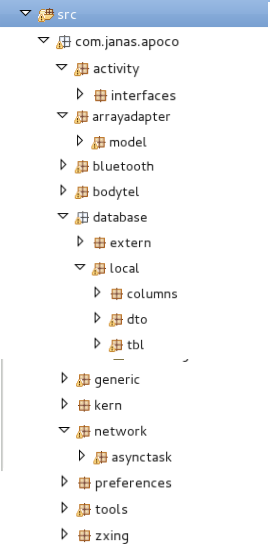
\includegraphics[scale=0.7]{screenshots/kapitel4/projekt_struktur/projekt_struktur_pakete.png}
%   \caption{Projekt-Paketstruktur der ApoCo-App}
%   
% \end{figure}
% 
% \subsection{Paket interfaces}
% 
% Im Paket Interfaces befinden sich Interface-Klassen welche das Zusammenspiel zwischen Activities und Objekten f\"ur Anwendungslogik unterstz\"utzen.
% Besonders wichtig ist hier der Zugriff auf bestimmte Objektmethoden und damit zusammenh\"angende Polymoorphie.
% Folgende Interfaces liegen im Paket vor:
% 
% \begin{itemize}
%  \item AccessableCreatorIF:\\
%  Dieses Interface dient zum erzeugen von unterschiedlichen Threads zur Kommunikation zwischen Software und externen Sensoren.
%  Dies gelingt durch Polymorphie.
%  F\"ur Jeden Sensor steht ein spezialisierter Thread zur kommunikation bereit.
%  \"Uber dieses Interface wird immer das richtige Objekt durch die jeweilige Activity erzeugt und weiter gereicht.
% 
%  \item ActivityExtrasCodesIF:\\
%  In Android ist es m\"oglich Objekte oder einzelne Werte zwischen den Activitys auszutauschen.
%  Daf\"ur sind in diesem Interface Konstanten f\"ur Benennung der Daten bereitgestellt, welche irgend wo in der ApoCo-App zwischen den Activities, 
%  \"uber den Intent-Extras-Mechanismus ausgetauscht werden.
%  \item ActivityRequestCodesIF:\\
%  Soll aus einer Activity eine weitere gestartet werden und erwatet man von dieser eine Antwort, so wird bei diesem Vorgang ein \emph{RequestCode} mitgegeben
%  der nach Ablauf einer Aufgabe als Antwort zur\"uck zur Urspr\"unglichen Activity zur\"uck kommt.
%  Mit diesem RequestCode kann die Activity unterscheiden welche Antwort sie gerade bekommen hat.
%  \item CloseableIF:\\
%  Eine Activity welche dieses Interface implementiert, darf zum Beispiel von einem Thread oder Handler geschlossen werden.
% %  \item MessageDisplayableIF:\\
%  \item WriteToPerformableIF:\\
%  Dieses Interface muss von einer Activity implementiert werden, wenn sie eine Nachricht \"uber Bluetooth versenden muss.
%  Die Nachricht wird an ein Thread \"ubergeben und dieser schreibt sie dann in den Streaminput eines BluetoothSocket.
% \end{itemize}
% 
% \subsection{Paket arrayadapter}
% 
% Im Paket arrayadapter befinden sich Implementierungen von performanten ArrayAdaptern.
% Werden Daten in einer ListView dargestellt so kann man sie bequem aus einem Container, mittels einem ArrayAdapter in die ListView laden.
% Die meisten Listen in ApoCo benutzen keine standard Darstellung von Daten in einer ListView sondern eine individuell zugeschnittene Version.
% F\"ur diesen Zweck ben\"otigt man einen zugeschnittenen ArrayAdapter dessen Funktionalit\"at implementiert werden muss.
% Die eigenen ArrayAdapter sind in der Lage Daten zwischenzuspeichern, wenn durch die ListView hin und her gescrollt wird.
% Diese Daten m\"ussen nicht mehr nachgeladen werden und das sorgt f\"ur bessere Performance.\\
% Im Paket arrayadapter befindet sich ein Unterpaket.
% Hier werden \emph{Model-Klassen} hinterlegt.
% Das sind Daten-Container welche Informationen f\"ur genau eine Messung speichern.
% Zus\"atzlich bietet jedes Model eine Static-Methode an um aus einem Datenobjekt, welches aus der Datenbank gelesen wurde, ein Objekt vom Typ des eigenen Model zu erzeugen.
% Jede ListView findet hier einen eigenen ArrayAdapter und das dazugeh\"orige Model.
% 
% \subsection{Paket bluetooth}
% 
% In diesem Paket befinden sich Klassen und Interfaces, welche sich um die Kommunikation \"uber Bluetooth k\"ummern.
% \begin{itemize}
%  \item AcceptThread:\\
%  Diese Klasse ist ein Thread, der einen BluetoothServerSocket startet und auf ankommende Anfragen zur Kommunikation wartet.
%  Das ist der erste Schritt von Kommuikationsaufbau.
%  
%  \item AccessableIF:\\
%  \"Uber dieses Interface kommunizieren Activities mit Threads, welche eine BluetoothSocket verbindung halten.
%  
%  \item BluetoothManager:\\
%  Der BluetoothManager soll die gesammte Funktionalit\"at um Bluetooth in einer Klasse vereinigen.
%  Mit dem BluetoothManager Objekt wird die Kommunikation aufgebaut, kontroliert und beendet.
%  
%  \item ConnectingThread:
%  Dieser Thread ist der zweite Schritt zur Kommunikation \"uber Bluetooth.
%  Er \"offnet einen Socket zur Gegenstelle und sendet Daten zwischen der Gegenstelle und der Activity.
%  
%  \item HandlerMessageIF:\\
%  Dieses Interface beinhaltet alle Konstanten f\"ur einen Nachrichtenaustausch \"uber einen Handler.
%  Die Konstanten erm\"oglichen der Activity zu erkennen wie sie mit der Nachricht umgehen soll.
%  
%  \item PairingThread:\\
%  Das ist ein Thread der keine Kommunikation aufbaut.
%  Er wird nur ganz kurz f\"ur das Koppeln von Smartphone und einem Sensor genutzt.
% 
%  \item StandardUUIDsIF:\\
%  Dieses Interface ist vorgesehen um bekannte standard UUIDs als Konstante bereitzustellen.
%  
%  \item StartableCanceableIF:\\
%  Dieses Interface schreibt einem Thread vor, dass er von Au\ss{}en gestartet und beendet werden kann.
% \end{itemize}
% 
% \subsection{Paket bodytel}
% 
% Dieses Paket beinhaltet alle Klassen und Interfaces die nottwendig sind um eine Kommunikation mit Ger\"aten
% der Firma Bodytel herzustellen.
% Im Augenblick werden die Sensoren WeightTel und PressureTel unterst\"utzt.
% 
% \begin{itemize}
%  \item BloodpressureResult:\\
%  Nach einer Blutdruckmessung wird aus dieser Klasse ein Objekt erzeugt und mit den Messwerten initialisiert.
%  Das Objekt wird anschliessend in ein Model- und ein DTO-Objekt, zum anzeigen in einer ListView und zum speichern in der Datenbank konvertiert.
%  
%  \item BodyTelUUIDsIF:\\
%  Dieses Interface stellt Konstanten bereit, welche von der Firma BodyTel als UUIDs f\"ur die Bluetoothverbindung genutzt werden.
%  
%  \item BodyweightResult:\\
%  Nach einer K\"orpergewichtsmessung wird aus dieser Klasse ein Objekt erzeugt und mit den Messwerten initialisiert.
%  Das Objekt wird anschliessend in ein Model- und ein DTO-Objekt, zum anzeigen in einer ListView und zum speichern in der Datenbank konvertiert.
%  
%  \item PressureTelConnectedThread:\\
%  Dieser Thread baut ein BluetootkSocket zwischen Smartphone und dem PressureTel-Blutdruckmesser auf.
%  
%  \item PressureTelCreator:\\
%  Eine Activity nutzt diese Klasse um den BluetoothManager mitzuteilen dass beim BluetoothVerbindungs-Aufbau ein Thread zur Kommunikation mit dem PressureTel gew\"unscht wird.
%  
%  \item PressureTelMeasurementDecoder:\\
%  Diese Klasse dekodiert eine Nachricht von dem Blutdruck-Sensor.
%  Daf\"ur wird die Nachricht in eiem \emph{PressureTelSMS}-Objekt gewrappt und alle Messungen die in der Nachricht enthalten sind als seperate \emph{BloodpressureResult}-Objekte
%  in einer \emph{List} zur\"uckgegeben.
%  
%  \item PressureTelMessageProtocol:\\
%  Ger\"ate der Firma BodyTel erwarten eine Art Konversations-Protokoll.
%  Um die Messwerte auszulesen muss dieses Protokoll erf\"ullt werden.
%  In diesem Interface werden die notwendigen Konstanten f\"ur die Kommunikation mit dem Sensor PressureTel bereitgestellt.
%  
%  \item PressureTelMessageReader:\\
%  Diese Klasse reagiert nach Protokoll auf Anfragen bei der Kommunikation mit dem PressureTel-Blutdrucksensor.
%  Sie nutzt die anderen PressureTel-Klassen um eine Nachricht zu analysieren, auf die zu antworten, Messwerte aus dieser zu dekodieren und sie in einer Liste an die Activity weiter zu geben. 
%  
%  \item PresurreTelSMS:\\
%  Diese Klasse ist eine Wraper-Klasse f\"ur eine SMS-Nachricht des PressureTel-Sensors.
%  Ein Objekt von dieser Klasse wird mit einer SMS initialisiert und konvertiert sie in ein f\"ur ApoCo verwendbares Format.
%  
%  \item WeightTelConnectedThread:\\
%  Dieser Thread baut ein BluetootkSocket zwischen Smartphone und der WeightTel-K\"orperwaage auf.
%  
%  \item WeightTelCreator:\\
%  Eine Activity nutzt diese Klasse um den BluetoothManager mitzuteilen dass beim BluetoothVerbindungs-Aufbau ein Thread zur Kommunikation mit dem WeightTel gew\"unscht wird.
%  
%  \item WeightTelMeasurementDecoder:\\
%  Diese Klasse dekodiert eine Nachricht von dem K\"orpergewicht-Sensor.
%  Daf\"ur wird die Nachricht in eiem \emph{WeightTelSMS}-Objekt gewrappt und alle Messungen die in der Nachricht enthalten sind als seperate \emph{BodyweightResult}-Objekte
%  in einer \emph{List} zur\"uckgegeben.
%  
%  \item WeightTelMessageProtocol:\\
%  In diesem Interface werden die notwendigen Konstanten f\"ur die Kommunikation mit dem Sensor WeightTel bereitgestellt.
%  
%  \item WeightTelMessageReader:\\
%  Diese Klasse reagiert nach Protokoll auf Anfragen bei der Kommunikation mit dem WeightTel-K\"orpergewichtssensor.
%  Sie nutzt die anderen WeightTel-Klassen um eine Nachricht zu analysieren, auf die zu antworten, Messwerte aus dieser zu dekodieren und sie in einer Liste an die Activity weiter zu geben.
%  
%  \item WeightTelSMS:\\
%  Diese Klasse ist eine Wraper-Klasse f\"ur eine SMS-Nachricht des WeightTel-Sensors.
%  Ein Objekt von dieser Klasse wird mit einer SMS initialisiert und konvertiert sie in ein f\"ur ApoCo verwendbares Format.
% \end{itemize}
% 
% \subsection{Paket Database}
% 
% Die Klassen und Interfaces in diesem Paket erm\"oglichen einen Zugriff auf die interne SQLite- und die externe MySQL-Datenbank.
% Im Unterpaket \emph{extern} befinden sich zwei Interfaces.
% Das Interface \emph{ExternServerDIR} hat eine Konstante mit dem Verzeichnis auf dem Webserver wo sich die REST-Schnittstelle zum MySQL-Datenbankserver befindet.
% Im Interface \emph{\texttt{PHP\_URL\_IF}} befinden sich Konstanten, welche PHP-URLs entsprechen.
% Diese URLs erf\"ullen jeweils eine Funktionalit\"at der REST-Schnittstelle des Webservers.
% Zum Beispiel entspricht die Konstante \emph{\texttt{REGISTER\_USER}} der URL \emph{\texttt{register\_user.php}}.
% Ruft ApoCo diese URL mit den notwendigen Parametern auf, so ist es m\"oglich einen neuen User im System anzulegen.\\
% 
% Im Unterpaket \emph{local} sind Interfaces und Klasse f\"ur die Interne Datenbank auf dem Smartphone.
% Das Paket beinhaltet weitere Unterpakete: \emph{column}, \emph{dto} und \emph{tbl}.
% Dies geh\"ohrt zu einem Objektorientierten Konzept zum Zugriff auf die Datenbank, welches in einem Separaten Kapitel erl\"autert wird.
% Des weiteren enth\"allt das Paket local die Klasse DBManagerLocal und das Interface DBManagerPreferencesIF.
% Der DBManagerLocal dient jeder Aktivity als Zugriffsmanager auf die interne Datenbank.
% Das Interface DBManagerPreferencesIF dient zum erstellen und der Konfiguration der Datenbank f\"ur die ApoCo-App.
% 
% \subsection{Paket generic}
% 
% In diesem Paket befinden sich drei Klassen f\"ur durchf\"uhrung einer W\"agemessung mit der Lebensmittelwaage.
% \begin{itemize}
%  \item GenericCreator:\\
%  Diese Klasse erzeugt einen Thread zur Kommunikation zwischen einer Activity und der KERN-PCB Laborwaage.
%  \item KcalConnectedThread:\\
%  Dieser Thread baut einen BluetoothSocket mit der Waage auf und kommuniziert mit ihr.
%  \item KcalResult:\\
%  Diese Klasse representiert einen Messwert der Laboorwaage kombiniert mit Informationen \"uber einem durch den Barcode erkannten Lebensmittel.
% \end{itemize}
% 
% \subsection{Paket kern}
% 
% In diesem Paket ist nur die Klasse \emph{\texttt{KERN\_PCB\_MessageBuilder}} enthalten.
% Die Kern-Laborwaage sendet eine Messung als Datenschnippsel.
% Diese Datenschnippsel werden in dieser Klasse gesammelt, analysiert und ein Messwert extrahiert.
% Eine Activity kann anschliessend \"uber die Methode \emph{readMessage()} den Messwert auslesen.
% 
% \subsection{Paket network}
% 
% Hier befinden sich alle Klassen und Interfaces die notwendig sind f\"ur eine Kommunikation \"uber WLAN oder das Mobile-Netz.
% \begin{itemize}
%  \item \texttt{JSON\_TAG\_IF}:\\
%  Dieses Interface stellt alle TAGs zu verf\"ugung, welche bei einem Datenaustausch mit dem Webserver im JSON-Format genutzt werden.
%  
%  \item NetworkHandler:\\
%  Diese Klasse ist ein Handler der in jeder Activity genutzt wird, welche mit dem Webserver kommunizieren muss.
%  Vor einem Datenaustausch wird \"uberpr\"uft ob eine WLAN- oder Mobile-Netz-Verbindung besteht und ob der Webserver antwortet.
%  Je nach Ergebnis reagiert der Handler und benachrichtigt den Benutzer wenn der Server nicht erreichbar ist.
%  Eine Activity kann von diesem Handler geschlossen werden.
%  Dazu muss sie das Interface CloseableIF implementieren und mit einem Flag best\"atigen.
%  Durch das Interface ist sie \emph{beenderbar} aber erst mit dem Flag wird dies auch abh\"angig von der Situation angefordert.
% \end{itemize}
% 
% Im Unterpaket \emph{asynctask} befinden sich Klassen welche von der Klasse \emph{AsyncTask<T,T,T>} abgeleited werden.
% Es handelt sich dabei um Threads, welche einen Teil der Arbeit im UI-Thread durchf\"uhren und den Hauptteil als Nebenl\"aufigkeit.
% Mit diesen Threads wird je eine bestimmte Netzwerk-Funktionalit\"at der ApoCo-App erledigt.
% 
% \subsection{Paket preferences}
% 
% Dieses Paket beinhaltet den \emph{PreferencesManager} und ein Interface \emph{\texttt{APOCO\_PREFERENCES}}.
% Der PreferencesManager behandelt ApoCo spezifische Parameter.
% Normalerweise k\"onnen Werte in einer Datei oder Datenbank persistent Gespeichert werden.
% \emph{Shared Preferences} ist eine weitere M\"oglichkeit in Android, Applikationsbezogene Werte als eine art \emph{Key-Value}-Paar zu speichern.
% Das Interface \texttt{APOCO\_PREFERENCES} beinhaltet alle \emph{keys} f\"ur den Zugriff auf die Schared-Preferences.
% 
% \subsection{Paket tools}
% 
% Das Paket tools beinhaltet Werkzeuge die Projekt\"ubergreiffend oder an mehreren Stellen im Projekt n\"utzlich sein k\"onnen.
% 
% \begin{itemize}
%  \item BloodpressureDiagnose:\\
%  Diese Klasse bietet Funktionen die eine einfache Interpretation von Blutdruckwerten \"ubern\"ahmen.
%  Man \"ubergibt Blutdruckwerte an die Methode \emph{performDiagnose()} und bekommt eine Aussage \"uber die Messung.
%   
%  \item BodyweightDiagnose:\\
%  Diese Klasse errechnet die Differenz zwischen Dem Zielk\"orpergewicht und dem Aktuellen K\"orpergewicht.
%  
%  \item ConnectivityTest:\\
%  Mit dieser Klasse ist es m\"oglich durch den Aufruf der Methode \emph{isAnyNetworkReachable()} festzustellen ob das Smartphone \"uber WLAN oder Mobile-Netz mit 
%  dem Internet verbunden ist.
%  
%  \item DateTemplateIF:\\
%  Dieses Interface enth\"allt Datum-Muster als Konstanten f\"ur eine Konvertierung eines Datums in ein Bestimmtes Format, welches durch das Muster vorgegeben wird.
%  
%  \item FloatPrecision:\\
%  Diese Klasse \"uberpr\"uft einen Flieskomawert ob er Nahe der Zahl Null liegt. F\"ur den Test ist ein Epsilon f\"ur die Prezision notwendig.
%  
%  \item HexConverter:\\
%  Diese Klasse bietet mehrere Methoden an um Hexadezimal-Codierte Bytearrays in lesbare String umzuwandeln und umgekehrt.
%  
%  \item JSONParser:\\
%  Diese Klasse erleichtert das Senden und Empfangen von JSON-Strings zwischen einer App und einem Webserver.
%  Dabei ist es m\"oglich die HTTP-Methoden POST und GET zu benutzen.
%  Die Serverantwort wird als JSON-Objekt zur\"uckgegeben.
%  
%  \item PasswordCheck:\\
%  Diese Klasse \"uberpr\"uft ob ein Passwort der gew\"unschten Vorgabe entspricht.
%  Es wird die Mindestl\"ange und die wiederhollte Eingabe des Passwortes gepr\"uft.
%  
%  \item ResourcesTools:\\
%  Diese Klasse ist ein Wraper um aus Android-Ressourcen eine String-Resource zu lesen.
%  
%  \item TimeTools:\\
%  Diese Klasse konvertiert einen Timestamp von Typ Long in einen String mit dem Format: \emph{dd-MM-yyyy HH:mm} und umgekehrt.
%  
%  \item Toasting:\\
%  Diese Klasse erleichtert Informationen mittels einen Toast anzuzeigen.
%  Der hier ausgegebene Toast entspricht nicht den standard Vorgaben sonden ist individualisiert.
%  
%  \item URLBuilder:\\
%  Diese Klasse bietet die Methode \emph{getURL()} an.
%  Mit dieser Methode wird aus Parametern und einem formatiertbaren String eine vollst\"andige URL-Adresse zusammen gef\"ugt.
% \end{itemize}
% 
% \subsection{Paket zxing}
% 
% Dieses Paket enth\"allt zwei Klassen.
% \emph{IntentIntegrator} und \emph{IntentResult}.
% Diese zwei Klassen sind notwendig um eine externe Barcode-Skanner-App zu nutzen.
% Die App wird mit der Unterst\"utzung dieser Klassen in die eigene App integriert und man erh\"allt Zugriff auf das den Barcode als String.



\section{Architektur der ApoCo-Datenbank(SQLite)}

Im Buch von Arno Becker und Marcus Pant\cite[S.244]{Android:02}, wird ein Architekturvorschlag f\"ur eine
Datenbankzugriffsschicht f\"ur Android-Anwendungen gemacht.
ApoCo folgt diesem Vorschlag, der hier erl\"autert wird.

\subsection{Motivation}

Beim Umgang mit einer Datenbank ist es oft erw\"unscht eine von der Anwendungsschicht getrennte Zugriffsschicht auf die Datenbank zu haben.
Daf\"ur kann man sich an dem Konzept der Programmierung mit Java-EE orientieren.
Android ist f\"ur ein solches Konzept nicht ausgelegt und so ergeben sich folgende Nachteile:

\begin{itemize}
 
\item Die Anwendung wird ungewollt gro\ss{} und die Performance sinkt.
\item Da keine Frameworks, wie zum Beispiel Spring oder Hibernate existieren, sind \"Anderungen an der Datenbank sehr aufwendig.
\item Es gibt keine M\"oglichkeit die Datenbankschicht von der Pr\"asentationsschicht ohne sp\"urbaren Leistungsabfall zur Laufzeit zu trennen
\cite[S.244]{Android:02}.

\end{itemize}

Au\ss{}erdem wurde festgestellt, dass eine reine Schichtentrennung unm\"oglich ist, 
wenn man mit einem Cursor-Objekt arbeiten m\"ochte.
Der Cursor ist wie ein Zeiger und ist darauf ausgelegt mit gro\ss{}en Datenmengen in einer Datenbank umgehen zu k\"onnen.\\

\subsection{Architekturumsetzung}

Die Zugriffsschicht auf die Android-Datenbank besteht aus den folgenden Klassen:

\begin{itemize}
 \item DBManagerLocal
 \item TabellennameColumns
 \item TabellennameDTO
 \item TabellennameTbl
\end{itemize}

Dabei ist zu beachten, dass f\"ur jede Tabelle eine \emph{Columns, DTO} und \emph{Tbl}-Klasse existiert. 
Die Bezeichnung dieser Klassen setzt sich aus dem Tabellennamen als Pr\"afix und den so eben genannten Klassenendungen zusammen.\\

Die Klasse \emph{DBManagerLocal} ist eine Verwaltungsklasse, um die Datenbank in der Activity greifbar zu machen.
Diese Verwaltungsklasse erweitert die Klasse SQLiteOpenHelper aus dem Android-SDK.
Der SQLiteOpenHelper wei\ss{} wie eine Datenbank erzeugt und ge\"andert wird.
Daf\"ur sind zwei Methoden vorgegeben: \emph{onCreate()} und \emph{onUpgrade()}.
Mit diesen zwei Methoden wird das Datenbankschema aufgebaut und bei \"Anderungen gel\"oscht und neu aufgebaut.
Um einen Backup-Mechanismus muss man sich selbst k\"mmern.
Des Weiteren sind im \emph{DBManagerLocal} Methoden implementiert, um mit der Datenbank Daten auszutauschen.
Im Listing 4.1 wird eine reduzierte Version des \emph{DBManagerLocal} implementiert und es wird eine Tabelle \emph{user} angelegt.
Die Klasse \emph{DBManagerLocal} implementiert die Schnittstelle \emph{DBManagerPreferencesIF}.
In dieser Schnittstelle wird der Name der Datei f\"ur die Datenbank und die Versionsnummer hinterlegt.
Die Versionsnummer ist hier sehr wichtig.
Wird das Datenbankschema ge\"andert, so muss die Versionsnummer inkrementiert werden.
Nur so erkennt die Klasse SQLiteOpenHelper, dass die Datenbank neu aufgebaut werden muss.\\

\begin{lstlisting}[caption={Beispiel f\"ur reduzierte Implementierung der \emph{DBManagerLocal} Klasse}]
 public class DBManagerLocal extends SQLiteOpenHelper implements DBManagerPreferencesIF{ 
 
    public DBManagerLocal(Context context) {
       super(context, DATENBANK_NAME, null, DATENBANK_VERSION);
    } 
    public void onCreate(SQLiteDatabase db) { 
    }    
    public void onUpgrade(SQLiteDatabase db, int oldVersion, int newVersion) {
    }
 }
\end{lstlisting}

Die \emph{TabellennameColumns}-Klassen sind als Schnittstellen und werden pro Tabelle angelegt.
Sie besitzen Konstanten f\"ur jede Spaltenbezeichnung der jeweiligen Tabelle.
Im Listing 4.2 wird ein Beispiel \emph{Columns-Klasse} f\"ur die Tabelle \emph{user} veranschaulicht.\\

\begin{lstlisting}[caption={Die Schnittstelle \emph{UserColumns}}]
 public interface UserColumns {
     static final String _ID      = "_id";
     static final String VORNAME  = "vorname";
     static final String NACHNAME = "nachname";
     static final String EMAIL    = "email";
     static final String PASSWORD = "password";
 }
\end{lstlisting}

Beim Zugriff auf die Tabelle \emph{user} wird im SQL-Statement \"uber die Konstanten der \emph{Columns-Klasse} auf die 
einzelnen Tabellenspalten zugegriffen.
In der Klasse \emph{TabellennameTbl} werden Schemainformationen und SQL-Statements als Konstanten vom Typ String bereitgestellt.
Die Klasse \emph{DBManagerLocal} nutzt die Schemainformationen, um eine Tabelle zu erzeugen.
Die SQL-Statements sind als Prepared Statements zu verstehen.
Das bedeutet, dass sie nur ein SQL-Statement-Muster ohne Parameter repr\"asentieren.
F\"ur Parameter wird das Fragezeichen (\emph{?}) als Platzhalter verwendet, 
das vor dem Zugriff auf die Datenbank durch einen echten Parameter ersetzt wird.
Das Listing 4.3 veranschaulicht mit der \emph{UserTbl} eine Tabellenschema-Klasse.\\

\begin{lstlisting}[caption={Die Klasse \emph{UserTbl}}]
 public final class UserTbl implements UserColumns {
 
    //Tabellenname
    public static final String TABLE_NAME = "user";
    
    //Create-Statement zum Anlegen der Tabelle
    public static final String SQL_CREATE = 
       "CREATE TABLE " + TABLE_NAME + "(" + 
      _ID + " INTEGER PRIMARY KEY AUTOINCREMENT," + 
      VORNAME + " TEXT NOT NULL," + 
      NACHNAME + " TEXT NOT NULL," + 
      EMAIL + " TEXT NOT NULL," + 
      PASSWORD + " TEXT NOT NULL" + ");";
      
   //Drop-Statement zum L\"oschen der Tabelle
   public static final String SQL_DROP = 
      "DROP TABLE IF EXISTS " + TABLE_NAME;
      
   //Beispiel-Statement, welches alle Benutzer mit dem gleichen Nachnamen zurueckgibt.
   //Der Nachname wird als Parameter uebergeben.
   public static final String STMT_GET_USER = 
      "SELECT * FROM " + TABLE_NAME + 
      "WHERE " + NACHNAME + "=?";
}
\end{lstlisting}

Listing 4.4 zeigt ein Beispiel, um die Tabelle \emph{user} zu erzeugen oder sie bei \"Anderungen des Datenbankschemas neu zu erzeugen.
Daf\"ur ruft die \emph{DBManagerLocal}-Klasse die Methode \emph{onCreate()} bzw. \emph{onUpgrade()} automatisch auf.\\

\begin{lstlisting}[caption={\emph{DBManagerLocal} erzeugt die Tabelle \emph{user}}]
 public void onCreate(SQLiteDatabase db) {  
    //erzeuge user-Tabelle
    db.execSQL(UserTbl.SQL_CREATE);
 }
    
 public void onUpgrade(SQLiteDatabase db, int oldVersion, int newVersion) {
    //loesche und erzeuge die user-Tabelle
    db.execSQL(UserTbl.SQL_DROP);
    onCreate(db);
 }
\end{lstlisting}

Beim Aufrufen des DROP- und CREATE-Statements muss wegen der Tabellenabh\"angigkeiten auf die richtige Reihenfolge geachtet werden.
Erstellt werden immer zuerst Tabellen ohne Fremdschl\"ussel und dann der Rest.
Die Tabellen werden in genau umgekehrter Reihenfolge wieder gel\"oscht.
Die \emph{TabellennameDTO}-Klassen sind einfache Container-Klassen und erm\"oglichen einen objektorientierten Umgang mit den Ergebnissen aus Datenbankanfragen oder 
das \"Ubergeben eines \emph{DTO}-Objekts an die Datenbank zum Speichern.
Im Listing 4.5 wird eine stark reduzierte \emph{DTO}-Klasse f\"ur die Tabelle \emph{user} veranschaulicht.
Die \emph{DTO}-Klassen haben Felder, die den Spalten der Tabelle entsprechen, welcher sie angeh\"oren.
Ein \emph{DTO}-Objekt kann auf verschiedene Arten entstehen.
Aus Parametern, die sich aus Messungen und Benutzereingaben ergeben, 
aus einer Datenbankanfrage, die einen Cursor liefert oder einem JSON-Objekt aus einer Anfrage an den Webserver.
Es kann auch notwendig sein ein Objekt mit einem Standardkonstruktor zu erzeugen und die Felder sp\"ater zu initialisieren.
F\"ur diese F\"alle werden vier Konstruktoren ben\"otigt.
Nicht jede \emph{DTO}-Klasse ben\"otigt immer alle vier Konstruktoren.\\

\begin{lstlisting}[caption={\emph{UserDTO}-Klasse in leicht reduzierter Form}]
public class UserDTO {

   public long _id;
   public String vorname;
   public String nachname;
   public String email;
   public String password;
   
   
   public UserDTO(){};
   public UserDTO(long, String, String, Sting, String){...}
   public UserDTO(Cursor){...}
   public UserDTO(JSONObject){...}
   //getter & setter
   
   public JSONObject toJSONObject() {... return jsonObj;}
}
\end{lstlisting}

Eine wichtige Methode jeder \emph{DTO}-Klasse ist die \emph{toJSONObject()}-Methode.
F\"ur den Fall, dass Messungen oder Benutzereingaben an den Webserver geschickt werden m\"ussen,
geschieht dies \"uber eine REST-Schnittstelle mit einem JSON-String.
Um es so einfach wie m\"oglich zu halten die Objekte als Parameter an die REST-Schnittstelle zu senden,
hat jedes Objekt die F\"ahigkeit seine gespeicherten Eigenschaften als ein JSON-Objekt zur\"uckzugeben.
Die Implementierung dieser Methode veranschaulicht das Listing 4.6.\\

\begin{lstlisting}[caption={\emph{UserDTO}-Klasse in leicht reduzierter Form}]
public class UserDTO {
   public JSONObject toJSONObject() {
      JSONObject obj = new JSONObject();
      try {
         obj.put(UserTbl._ID, this._id);
         obj.put(UserTbl.VORNAME, this.vorname);
         obj.put(UserTbl.NACHNAME, this.nachname);
         obj.put(UserTbl.EMAIL, this.email);
         obj.put(UserTbl.PASSWORD, this.password);
      } catch (JSONException e) {
         Log.d(CLAZZ_NAME, "toJSONObject failed: " + e.getMessage());
      }
      return obj;
   }
}
\end{lstlisting}
Das Listing 4.6 demonstriert auch gleichzeitig wie die \emph{Tbl}-, \emph{Columns}- und \emph{DTO}-Klassen zusammenarbeiten.
Um die richtige Spaltenbezeichnung zu nutzen, greift die \emph{DTO}-Klasse \"uber die \emph{Tbl}-Klasse auf die \emph{Columns}-Schnittstelle 
und dort auf die Konstanten der Spaltennamen zu.
Damit eine Activity mit dem \emph{DBManagerLocal} auf die Datenbank Zugriff bekommt, 
m\"ussen Methoden f\"ur den Zugriff in der Klasse \emph{DBManagerLocal} implementiert werden.
Im Listing 4.3 wird bereits das SQL-Statement \emph{\texttt{STMT\_GET\_USER}} in der \emph{UserTbl}-Klasse gezeigt.
Dieses Statement nutzt der \emph{DBManagerLocal} in einer eigenen Methode, um eine Anfrage daraus zu bauen.
Eine Beispielanfrage wird mit dem Listing 4.7 demonstriert.\\

\begin{lstlisting}[caption={Methode \emph{getUserByNachname()} der \emph{DBManagerLocal}-Klasse}]
public class DBManagerLocal ... {
   ...
   //Methode fuer eine Datenbankanfrage
   public Cursor getUserByNachname(UserDTO user) throws SQLException{
      //Hier wird der Nachname aus dem DTO-Objekt als Parameter in einem String-Array gespeichert.
      String[] param = {user.nachname};
      //getReadableDatabase liefert eine Referenz auf ein Objekt, welches die Datenbankverbindung zum Lesen oeffnet.
      //das Statement aus der Klasse UserTbl und die Parameter werden an die Methode rawQuery uebergeben.
      //rawQuery liefert einen Cursor auf die Antwort aus der Datenbank.
      Cursor cursor = getReadableDatabase().rawQuery(UserTbl.STMT_GET_USER, param);
      return cursor;
   }   
}
\end{lstlisting}

Das Ergebnis der Anfrage kann in einer Activity anschlie\ss{}end ausgewertet werden.
Eine Demonstration liefert das Listing 4.8.
Hier wird zuerst mit dem if-Statement gepr\"uft, ob ein Ergebnis in der Datenbank gefunden wurde.
Die while-Schleife bewegt beim ersten Durchlauf den Cursor auf die erste Zeile der Antwort.
Im Rumpf der while-Schleife werden die Ergebnisse bearbeitet, und das so lange bis die Methode moveToNext() ein false liefert.\\

\begin{lstlisting}[caption={Methode \emph{getUserByNachname()} der \emph{DBManagerLocal}-Klasse}]
public class MyActivity... {
   ...    
   DBManagerLocal dbManager = new DBManagerLocal(MyActivity.this);      
   
   public void todo() {         
      Cursor result = dbManager.getUserByNachname(user);      
      if (result.getCount() > 1) {      
         while(result.moveToNext()) {         
            UserDTO user = new UserDTI(result); ...
         }
      }
   }
}
\end{lstlisting}

\subsection{ApoCo Datenbankdiagramm}

In der Abbildung 4.4 wird das ApoCo Datenbankschema als Klassendiagramm dargestellt.
Die Abk\"urzungen \emph{FK1, FK2} stehen dabei f\"ur Fremdschl\"ussel. Die Prim\"arschl\"ussel werden als Schl\"usselsymbol dargestellt.
Folgende Tabellen sind im Diagramm zu sehen:

\begin{itemize}
 \item user:\\
 Diese Tabelle enth\"alt Daten der Patienten.
 Die ApoCo-Anwendung ist so konzipiert, dass sie mehrere Patienten auf einem Smartphone verwalten kann.
 Jeder Patient hat seine eigenen Anmeldedaten und kann die Daten der anderen Patienten nicht einsehen.
 
 \item bloodpressure:\\
 In dieser Tabelle werden Messprotokolle f\"ur den Blutdruck persistent gespeichert.
 Neben dem Datum und den Spalten f\"ur die Messwerte ist hier noch eine weitere Spalte mit der Bezeichnung \emph{sync} zu sehen.
 Diese Spalte ist f\"ur die Synchronisation der Daten mit dem Webserver norwendig.
 Es handelt sich dabei um einen Flag der von 0 auf 1 gesetzt wird, wenn die Messwerte an den Webserver \"ubertragen wurden.
 
 \item bodyweight:\\
 Die Tabelle \emph{bodyweight} speichert Messdaten zum K\"orpergewicht.
 Auch hier ist ebenfalls eine Flag-Spalte f\"ur den Synchronisationsvorgang.
 
 \item mealenergy:\\
 Die Tabelle \emph{mealenergy} repr\"asentiert pro Eintrag eine ganze Mahlzeit.
 Hier wird nur festgehalten wann die Mahlzeit eingenommen wurde und ob die Mahlzeit mit dem Webserver synchronisiert ist.
 
 \item \texttt{mealenergy\_content}:\\
 Diese Tabelle enth\"alt einzelne Positionen einer Mahlzeit.
 Sie speichert aber nur das Gewicht und die Energiemenge der jeweiligen Position, wie auch die dazugeh\"orige EAN-Nummer.
 Die Tabellen \emph{mealenery} und \emph{\texttt{mealenergy\_content}} bilden somit eine Einheit bei der Berechnung von Energieaufnahme 
 durch die Nahrung.
 
 \item food:\\
 Die Tabelle \emph{food} dient als Erg\"anzung der Positionen einer Mahlzeit.
 Jedes Lebensmittel, das zum ersten Mal mit Hilfe des Barcodescanners erkannt wurde, wird hier f\"ur schnellen Zugriff gespeichert.
 
 \item tageseinheiten:\\
 Der Arzt gibt seinen Patienten vor, wieviel Kilokalorien sie am Tag zu sich nehmen d\"urfen.
 Die aktuellen Werte werden vom Webserver geladen und in dieser Tabelle abgelegt.
\end{itemize}

\begin{figure}[h]
  \centering
  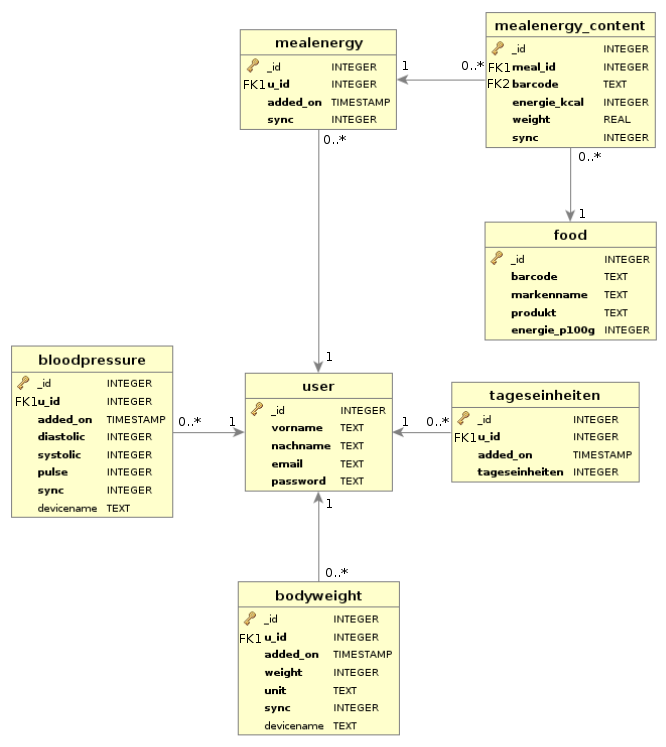
\includegraphics[scale=0.53]{diagramme/kapitel4/apoco_datenbank_schema.png}
  \caption{ApoCo Datenbankdiagramm}
  
\end{figure}

% \section{Architektur der ApoCo-Datenbank(SQLite)}
% 
% blabla \cite[S.244]{Android:02}





\section{ApoCo Use Cases}

\subsection{Use Case- Diagramm}

Die Abbildung 4.11 veranschaulicht ein Use Case-Diagramm der ApoCo-Anwendung.
Hier werden Interaktionsm\"oglichkeiten des Benutzers mit der Android-Anwendung und die Kommunikation 
mit dem Webserver abgebildet.
\begin{figure}[h]
  \centering
  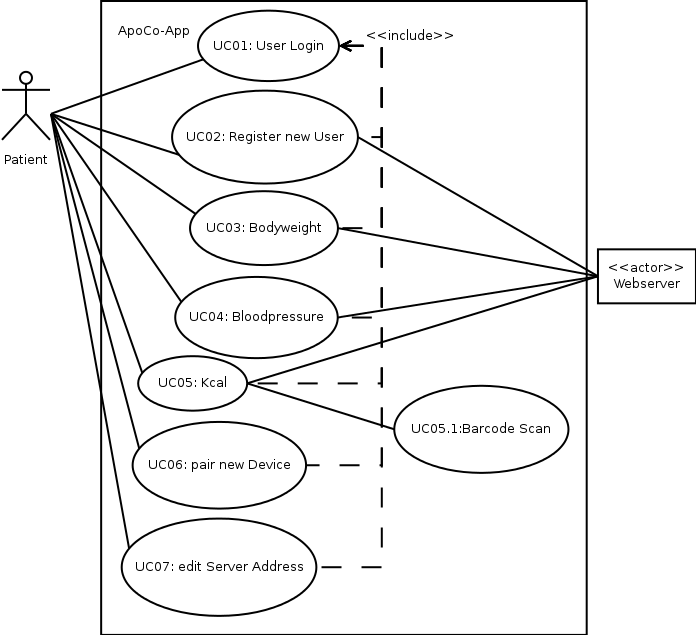
\includegraphics[scale=0.6]{diagramme/kapitel4/use_cases.png}
  \caption{ApoCo Use Case-Diagramm}
  
\end{figure}

\subsection{Aktoren}

\begin{itemize}
 \item Patient: Benutzer der ApoCo-Anwendung
 \item Webserver: Webserver mit Service zur Verwaltung der Tagesprotokolle
\end{itemize}

\subsection{Use Case Kurzbeschreibungen}

\begin{itemize}
 \item UC01: User Login\\ 
 Der Benutzer Meldet sich bei der ApoCo-Anwendung an.
 \item UC02: Register new User\\ 
 Ein neuer Benutzer registriert sich im System.
 Die Benutzerdaten werden zum Server gesendet und von diesem erlaubt oder verweigert.
 \item UC03: Bodyweight\\ 
 Der Benutzer f\"uhrt eine K\"orpergewichtsmessung durch.
 Zielgewicht wird vom Server geladen.
 Die Messung wird an den Server gesendet.
 \item UC04: Bloodpressure\\ 
 Der Benutzer f\"uhrt eine Blutdruckmessung durch.
 Die Messung wird an den Server gesendet.
 \item UC05: Kcal\\ 
 Der Benutzer f\"uhrt eine Protokollierung seiner Mahlzeit durch.
 Informationen zum Lebensmittel werden vom Webserver geladen.
 Mahlzeitprotokoll wird an den Server gesendet.
 \item UC05.1: Barcode Scan\\ 
 Der Benutzer scannt w\"ahrend einer Mahlzeitprotokollierung ein Lebensmittel mittels Barcodescanner ein.
 \item UC06: Pair new Device\\ 
 Der Benutzer f\"uhrt eine Ger\"ate-Koppelung durch.
 \item UC07: edit Server Address\\ 
 Der Benutzer konfiguriert die Webadresse des Servers.
\end{itemize} 


% \section{ApoCo Use Cases}
% 
% \subsection{Use Case- Diagramm}
% 
% Die Abbildung 4.3 veranschaulicht ein Use Case- Diagramm der ApoCo-App.
% Hier werden Interaktionsm\"oglichkeiten des Benutzers mit der Android-App und die kommunikation mit dem Webserver abgebildet.
% \begin{figure}[h]
%   \centering
%   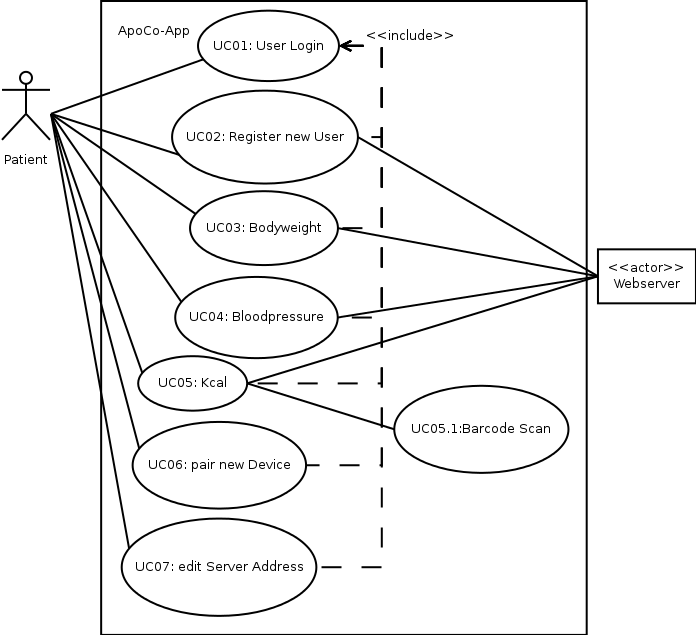
\includegraphics[scale=0.55]{diagramme/kapitel4/use_cases.png}
%   \caption{ApoCo Use Case- Diagramm}
%   
% \end{figure}
% 
% \subsection{Aktoren}
% 
% \begin{itemize}
%  \item Patient: Benutzer der ApoCo-App
%  \item Webserver: Webserver mit Service zur Verwaltung der Tagesprotokolle
% \end{itemize}
% 
% \subsection{Use Case Kurzbeschreibungen}
% 
% \begin{itemize}
%  \item UC01: User Login\\ 
%  Der Benutzer Meldet sich an der ApoCo-App an.
%  \item UC02: Register new User\\ 
%  Ein neuer Benutzer Registriert sich im System.
%  Die Benutzerdaten werden zum Server gesendet und von diesem erlaubt oder verweigert.
%  \item UC03: Bodyweight\\ 
%  Der Benutzer f\"uhrt eine K\"orpergewichtsmessung durch.
%  Zielgewicht wird vom Server geladen.
%  Die Messung wird an den Server gesendet.
%  \item UC04: Bloodpressure\\ 
%  Der Benutzer f\"uhrt eine Blutdruckmessung durch.
%  Die Messung wird an den Server gesendet.
%  \item UC05: Kcal\\ 
%  Der Benutzer f\"uhrt eine Protokolierung seiner Mahlzeit durch.
%  Informationen zum Lebensmittel werden vom Webserver geladen.
%  Mahlzeitprotokol wird an den Server gesendet.
%  \item UC05.1: Barcode Scann\\ 
%  Der Benutzer Skannt w\"ahrend einer Mahlzeitprotokolierung ein Lebensmittel mittels Barcode-Skanner ein.
%  \item UC06: Pair new Device\\ 
%  Der Benutzer f\"uhrt ein Ger\"ate-Pairing durch.
%  \item UC07: edit Server Address\\ 
%  Der Benutzer konfiguriert die Web-Adresse des Servers.
% \end{itemize}


\section{FUCK}


 F\"ur jede Messung wird eine andere Sensorart ben\"otigt und diese Sensoren benutzen jeweils ein eigenes Protokol zur Kommunikation.
 \"Uber dieses Interface wird daf\"ur gesorgt dass f\"ur die jeweilige Messung immer der entsprechende Thread erzeugt wird, welcher \"uber das entsprechende
 Protokol des Sensors 
 Dieses Interface dient der Polymorphie.
 Als \emph{Accessable} wird ein Thread angesehen der ein Socket \"uber Bluetooth zum Sensor aufbaut.
 Accessable hat hier die Bedeutung, die Activity hat zugrif auf den Thread.
 Um das zu verdeutlichen wird das im Listing 4.1 verdeutlicht.
 Die Activity \emph{ActivityBloodpressure} ruft nach dem sie gestartet wurde irgend wann ihre Methode \emph{onStart()} auf.
 In dieser Methode wird die Klasse \emph{BluetoothManager} verwendet, um einen \emph{BluetoothServerSocket} zu starten, welcher auf einkommende Nachrichten
 von gekoppelten Sensoren h\"ohrt.
 Der BluetoothManager bietet f\"ur diesen Vorgang die Methode \emph{listenForInquiryConnections()} an und
 muss nach der Verbindung daf\"ur sorgen dass mit dem entsprechenden Messsensor kommuniziert wird.
 F\"ur Blutdruck eben ein Blutdrucksensor.
 Damit das funktioniert wird das AccessableCreatorIF Interface benutzt, welches von der jeweiligen Activity an den BluetoothManager \"ubergeben wird.
 Es referenziert ein Objekt vom gew\"unschten Typ, von dem die Activity erwartet, dass es f\"ur Kommunikation mit dem richtigen Sensor sorgt.\\
 
 \begin{lstlisting}[caption={Beispiel f\"ur ein einfaches HTML-Dokument}]
 class ActivityBloodpressure { ... 
    protected synchronized void onCreate() { ...
       BTManager.listenForInquiryConnections(
         mBloodpressureHandler
         ,new PressureTelCreator()  //AccessableCreatorIF
         ,BodyTelUUIDsIF.PRESSURETEL_UUID_SPP_1234,
         SDP_SERVICE_NAME);
    }
 }
 //implementiert AccessableCreatorIF
 class PressureTelCreator implements AccessableCreatorIF { ...
   public AccessableIF createAccessable(...) {
      PressureTelConnectedThread connectedTask = null; ...
      return connectedTask;
   } 
 }
\end{lstlisting}

%%%%%%%%%%%%%%%%%%%%%%%%%%%%%%%%%%%%%%%%%%%%%%%%%%%%%%%%%



\section{ApoCo-GUI Gestaltung}

So weit es von der Funktionalit\"at der einzelnen Activity zugelassen, sind alle Activities identisch strukturiert.
Sie bestitzen immer die Elemente Header, Title, Body und Footer.
Das einhalten der Struktur soll durch ein einheitliches Layout eine angen\"ahme und einfache Bedienung der Software erm\"oglichen.
Die Abbildung 4.3 veranschaulicht und bennent die Haupt-Struktur-Elemente einer Activity an hand der Start-Activity der ApoCo-App.

\begin{figure}[h]
  \centering
  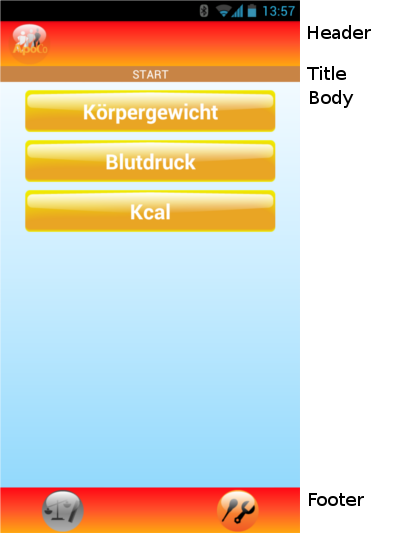
\includegraphics[scale=0.5]{screenshots/kapitel4/gui/activity_struktur.png}
  \caption{Start-Activity als Beispiel f\"ur Strukturierung}
  
\end{figure}

Die Struktur-Elemente haben jeweils eine eigene Funktion.
Im \emph{Header} ist immer das ApoCo-Logo und wenn notwendig ein \emph{Back-Button} angebracht.
Der Title bereich informiert den Benutzer immer auf welcher Activity er sich im Augenblick befindet.
Im Body sind Interaktions-Elemente oder weitere notwendige Informationen der aktuellen Activity angebracht.
Das k\"onnen Buttons zum ansto\ss{}en von Messvorg\"angen oder ListViews sein.
Eine ListView informiert den Benutzer \"uber alle bereits verzeichnette Messungen in der entsprechenden Activity.
Ganz Unten am Ende der Activity ist der Footer.
Er beinhaltet Buttons, mit dennen man in die Bereiche zum Ger\"ate-Pairing, Sprung zur Start-Activity und zur Server-Konfiguration gelangt.

\subsection{Bedienelemente}
Der Back-Button ist eines der Interaktions-Elemente welches den Benutzer zu der vorherigen Activity bringt.
Die Abbildung 4.4 veranschaulicht einen Header mit Back-Button.

\begin{figure}[h]
  \centering
  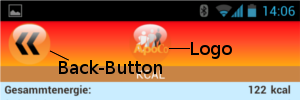
\includegraphics[scale=0.5]{screenshots/kapitel4/gui/header_backbtn.png}
  \caption{Header einer Activity mit Back-Button}
  
\end{figure}



Neben dem Back-Button gibt es noch weitere M\"oglichkeiten zu der vorhergehenden Activity zur\"uck zu kehren.
Einige davon haben ledeglich die Funktionalit\"at \emph{zur\"uck und Daten verwerfen} und andere wiederrum \emph{zur\"uck und Daten speichern}.
Die Abbildungen 4.5 und 4.6 veranschaulichen alle M\"oglichkeiten.

\begin{figure}[h]
  \centering
  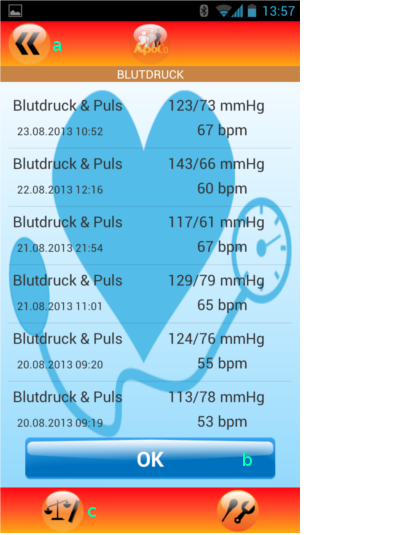
\includegraphics[scale=0.5]{screenshots/kapitel4/gui/back_btns.png}
  \caption{Zur\"uck-M\"oglichkeiten einer Activity}
  
\end{figure}

Die Abbildung 4.5 zeigt die Activity f\"ur Blutdruckmessung.
Hier sind die Buttons mit Buchstaben von \emph{a} bis \emph{c} gekennzeichnet.
\begin{itemize}
 \item a) Back-Button, Daten werden nicht gespeichert, zur\"uck zu vorherigen Activity. 
 \item b) OK-Button, Daten werden gespeichert, anschliessend zur\"uck zu vorherigen Activity.
 \item c) Start- oder Messung-Auswahl-Activity, Sprung aus jeder Activity zur\"uck zur Start-Activity. Daten werden nicht gespeichert. 
\end{itemize}

\begin{figure}[h]
  \centering
  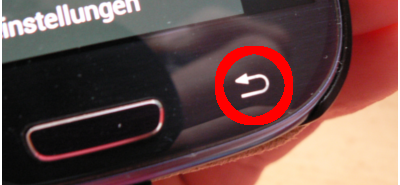
\includegraphics[scale=0.5]{screenshots/kapitel4/gui/hd_backbtn.png}
  \caption{Zur\"uck mit einem dem Hardware-Button des Smartphones}
  
\end{figure}

Der mit einem roten Kreis gekennzeichnete Hardware-Button des Smartphones f\"ur \emph{Zur\"uck}, wird in ApoCo wie der Back-Button implementiert.
Hier findet kein Speichern der Daten statt.
Befindet man sich in der Start-Activity beendet ein Dr\"ucken auf den Hardware-Taste die ApoCo-App.\\


\subsection{Funktionsweise von ApoCo}

Um ein Tagesprotokol aufzeichnen zu k\"onnen sind mehrere Schritte notwendig.
\begin{itemize}
 \item Der Patient registriert sich einmallig im System.
 \item Der Patient meldet sich mit ApoCo an.
 \item Die f\"ur die Messungen notwendige Hardware wird einmallig \"uber Bluetooth mit dem Smartphone bekannt gemacht. Das so genannte \emph{Pairing}.
 \item Eine Messung wird ausgew\"ahlt und die f\"ur sie vorgesehene Hardware genutzt.
 \item Die abgeschlossene Messung wird mit dem Server synchronisiert.
\end{itemize}

\subsubsection{Activitie-Map und Aufruf-Struktur}

\begin{figure}[h]
  \centering
  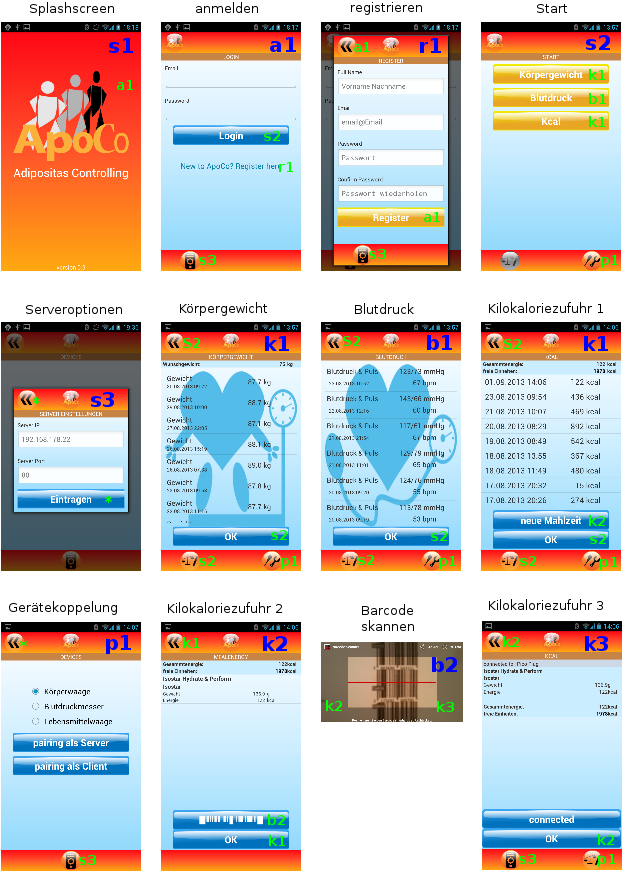
\includegraphics[scale=0.35]{diagramme/kapitel4/activity_map.png}
  \caption{Zur\"uck mit einem dem Hardware-Button des Smartphones}
  
\end{figure}


\subsection{Model}

\subsection{View}
\subsection{Controller}

\section{Vorgehensmodell}

Ein Teil der Funktionalit\"at wurde bereits im Praxissemester erarbeitet. 
Die Bacherlorarbeit erweitert die Ergebnisse aus dem Praxissemester.
Teilweise wurden die Ergebnisse zum Zweck der Erweiterung refaktoriert.
Es wurde ein Iteratives- und Inkrementeles- Vorgehensmodell einges\"atzt.

\section{Funktionale Anforderungen}



 
